\section{Introduction}
Internet of Things (IoT) is one of the research and industrial fields that faced a rapid growth in the recent years.
The approach to such ecosystem has been heterogeneous and sparse, leading to a wide variety of standards and solutions at each layer of the network and application stack.
It has been a source of interest from many different points of view, in such a way that now we have dedicated infrastructures at physical, data link, network, transport and application layers.
\\

Since the beginning of its diffusion, its potential has been explored in various fields of application and its major usefulness has been claimed to be in service composition and interoperability \cite{atzori2010internet}.

The requirements when designing collaborative IoT-related automation systems are varying due to the heterogeneity of the platforms and the hardware components as well as the network interfaces.
This resulted in a sparse set of technologies and terminologies used in several scenarios determining a lack of interoperability among systems.
The common approach to the problem of unifying entities within an ecosystem is typically architectural and leads to a difficult reuse of the components among different solutions \cite{krco2014designing}.
To face these issues the European Commission supported initiatives like IoT-A \cite{iot-a}, which aimed to release an architectural reference model and FI-WARE \cite{fiware}, which also helped architects in establishing an unified vision and nomenclature and now had become an implementation-driven open community.
It also provided a sandbox in which partners could upload their open data, however it is not of broad use nowadays.
However, such solutions did not solve the problem introduced by architectures, in fact different solutions tend to create separate islands which are hard to unify.
\\

In this paper we aim to show the usefulness and the potential of open data exploitation for global cooperative IoT automation scenarios.
As a preliminary approach, we focused our analyses on data coming from two of the main open data platforms for sensors: ThingSpeak and SparkFun.
Such platforms can be queried for data streams, supplied with a set of metadata, which gave us the motivation for such proposal.
In fact, raw data streams come with temporal information, especially regarding the stream creation date and last update date.
Such parameters can tell us much about the general trend in the usage of these platforms throughout a time window of few years.
Each stream in ThingSpeak comes with a creation date, which we reported, after a data extraction, in the diagram in figure~\ref{creationtrend}.
\begin{figure}[!b]
\centering
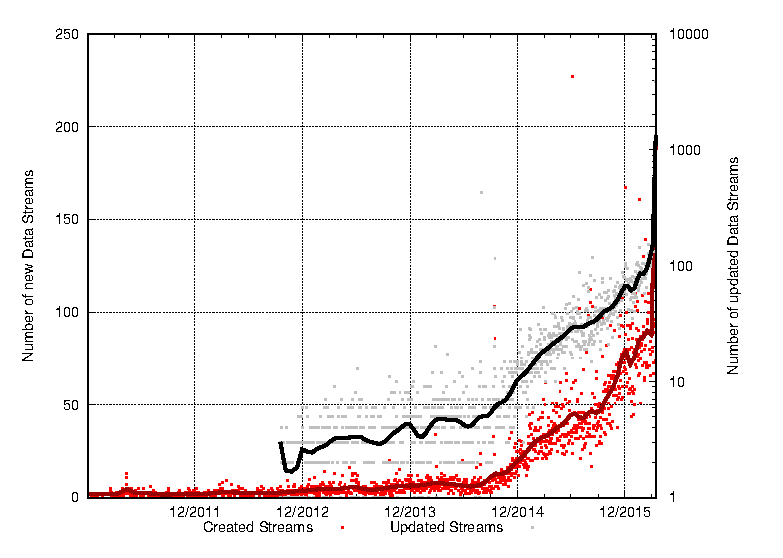
\includegraphics[width=0.50\textwidth]{img/bars.eps} 
\caption{Trend in creation of ThingSpeak channels.}
\label{creationtrend}
\end{figure}
Starting from such analysis it results a substantial growth in created channels.
Some of the steeper slopes are probably justifiable.
A possible intuition behind them is the parallel innovation in simple hardware modules, for instance August 2014 corresponds to the launch of the first version of ESP8266 \cite{esp8266} on the market and in October 2014 was possible to flash its firmware though an SDK \cite{espressif}.
Such period has not surprisingly been affected by a rapid growth according to the diagram. [TODO MORE EXAMPLES]
The diagram reports also the last update date for each stream.
It is immediately clear that, since the oldest update date is in September 2012 while the oldest creation date is in 2010, all the data streams created before 2012 that did not perform an update after such date have been deleted due to a certain policy.
The steepness of the curve in the last days reveals that a significant amount of the data streams are still in use and updated daily or even hourly.
\\

Such analyses shed some light on how rapidly the world of open data is growing and people are gaining interest in using a platform that takes away the burden of creating a local ecosystem.
Thus, our work creates the basis for a solid global ecosystem with a strong impact on cooperative services.